%
% För att skapa presentationer med LaTeX.
%
\documentclass[dvipsnames]{beamer}
% PSTricks och göm stolpmanus:
%\documentclass[xcolor=pst,dvips,notes=hide]{beamer}

\usepackage[T1]{fontenc}
\usepackage[swedish]{babel}
%\usepackage[latin1]{inputenc}
%\usepackage{times}
\usepackage{uu}
\usepackage{graphics}
\usepackage{hyperref}
\usepackage{lmodern}
\usepackage{multirow}
%\usepackage[dvipsnames]{xcolor}
\usepackage{colortbl}

\bibliographystyle{acl}

\newcommand{\icite}[1]{\structure{{\footnotesize \cite{#1}}}}
\newcommand{\ssicite}[1]{\structure{{\scriptsize \cite{#1}}}}
\newcommand{\argmax}{\operatornamewithlimits{argmax}} 
\newcommand{\argmin}{\operatornamewithlimits{argmin}} 

\title{Natural Language Processing} \subtitle{Introduction}
\author{Fabienne Cap, Miryam de Lhoneux and Joakim Nivre}
\institute{Uppsala University\\Department of Linguistics and
  Philology\\nlp-course@stp.lingfil.uu.se\\\vspace{0.5cm}Thanks to
  Joakim Nivre for designing and providing most of these slides!}
\logo{\includegraphics[height=1.25cm,clip=true,trim=0 30 0
  0]{UU_logo_vit_60}}

\begin{document}

\frame[c]{\titlepage}

\begin{frame}
\frametitle{What is NLP?}
\begin{itemize}
\item We study what it takes to make computers perform useful and interesting tasks involving human language
\item We are also interested in the insights that we can gain about human language from the study of computational models
\end{itemize}
\end{frame}

\begin{frame}
\frametitle{Showcase question answering: IBM's Watson}
\begin{itemize}
\item On February 16, 2011, IBM's computer system Watson defeated the world's best human Jeopardy champions
\end{itemize}
\begin{center}
\href{https://www.youtube.com/watch?v=P18EdAKuC1U}{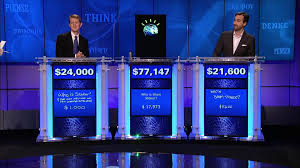
\includegraphics[scale=0.4]{watson}}
\end{center}
\end{frame}

% \begin{frame}
% \frametitle{Information extraction}
% \only<1>{\vspace{0.13cm}}
% \noindent
% %\hspace{-0.5cm}
% \only<1>{\hspace{-0.43cm}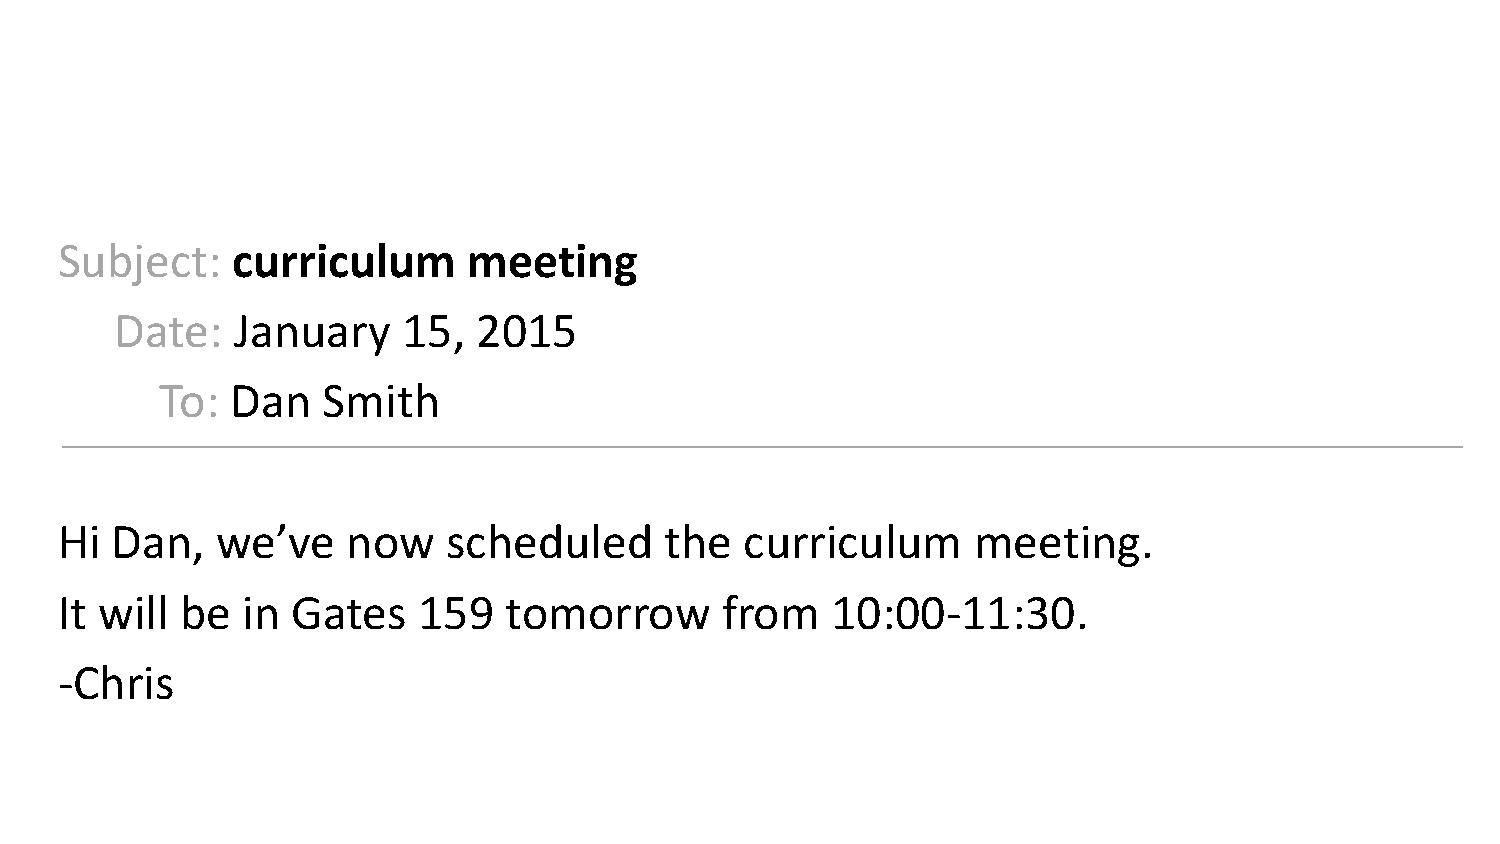
\includegraphics[scale=0.45]{ie1}}
% \only<2>{\hspace{-0.5cm}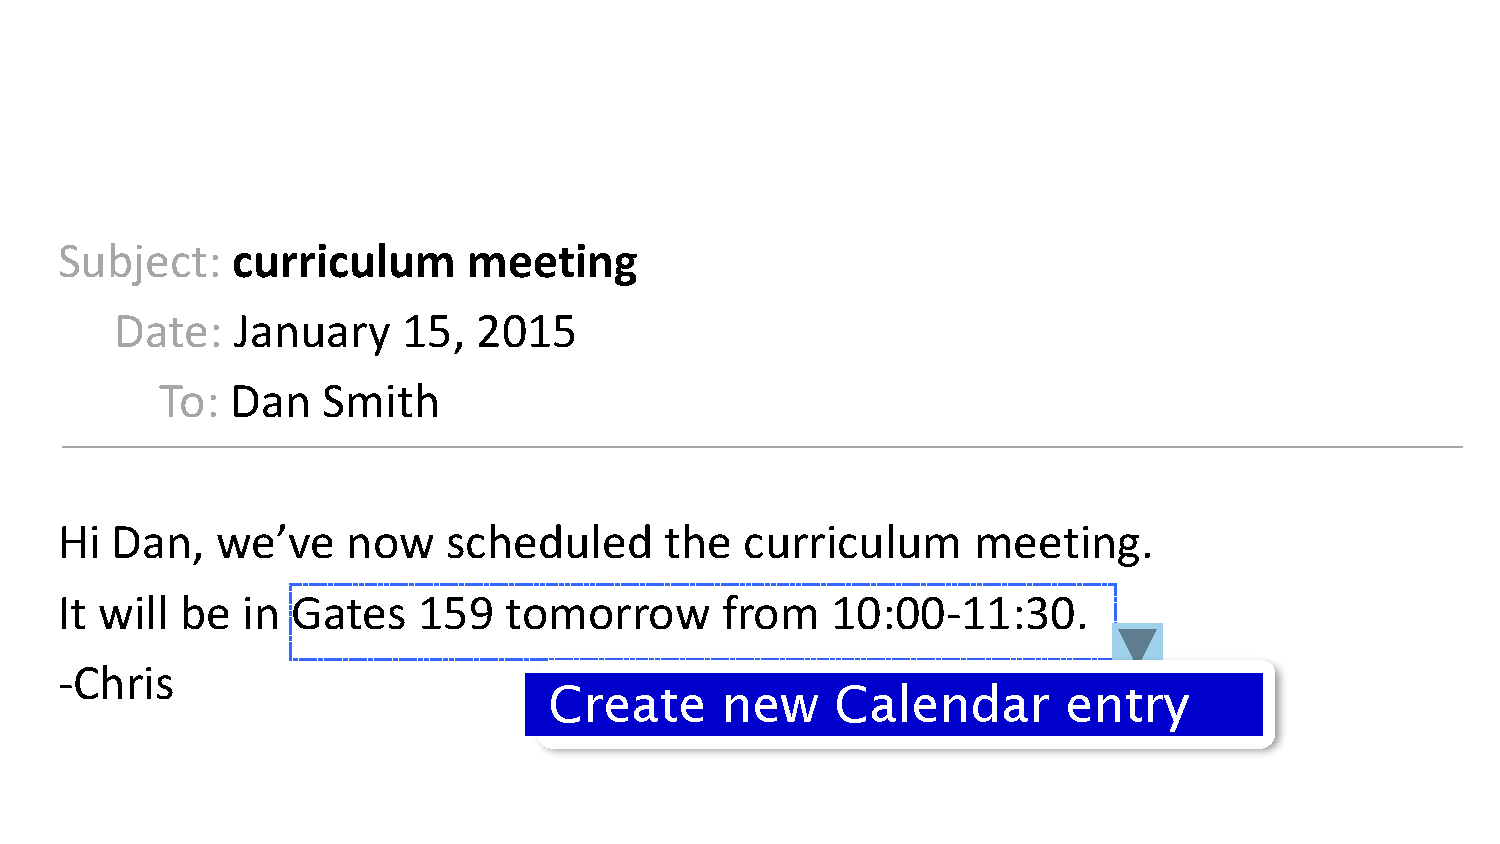
\includegraphics[scale=0.45]{ie2}}
% \only<3>{\hspace{-0.59cm}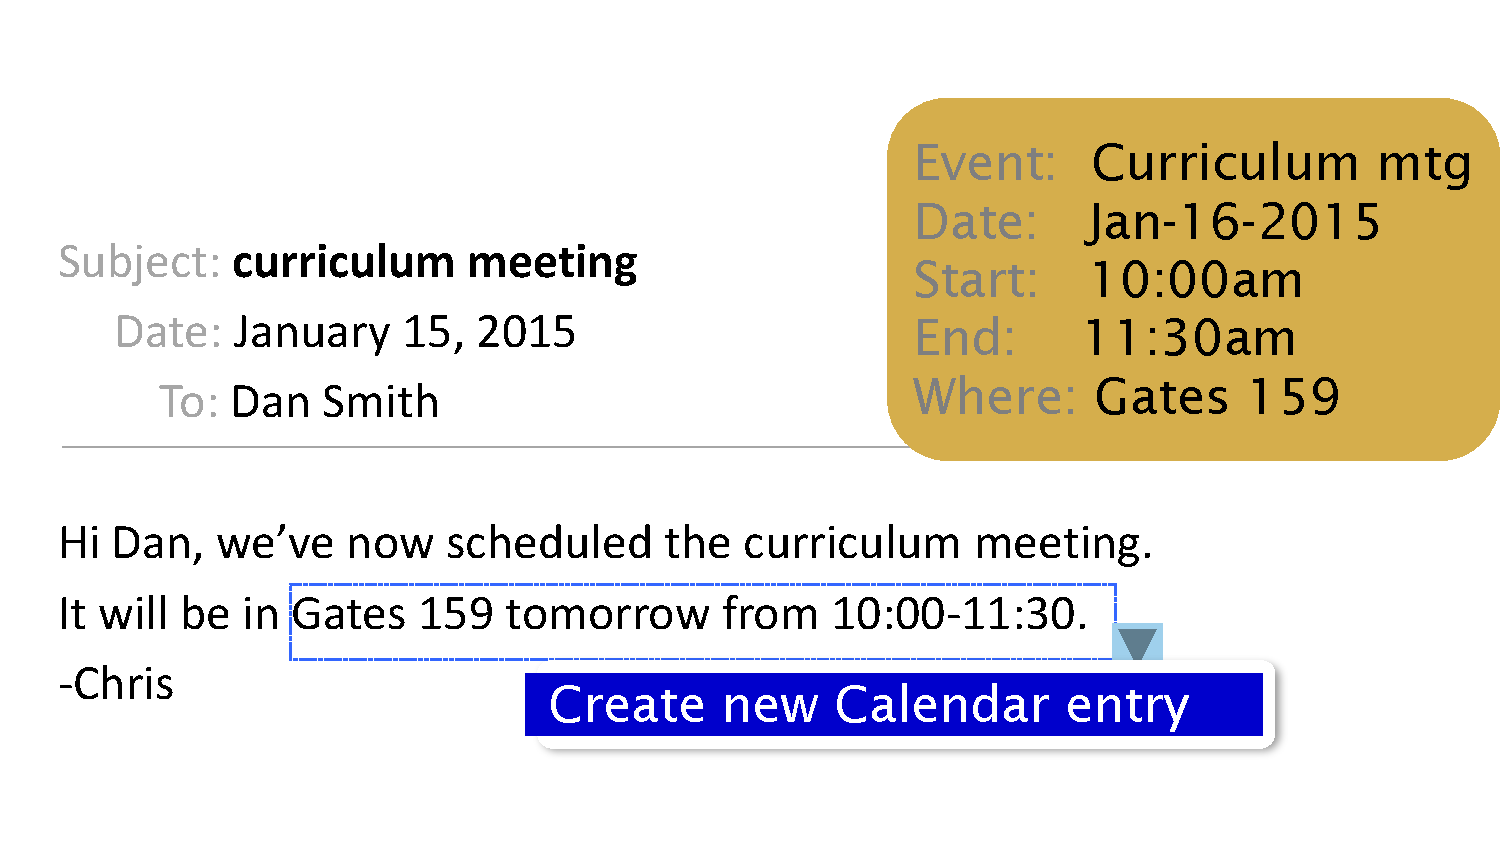
\includegraphics[scale=0.45]{ie3}}
% \end{frame}

% \begin{frame}
% \frametitle{Sentiment analysis}
% \only<1>{\vspace{0.095cm}}
% \only<3>{\vspace{-0.02cm}}
% \noindent
% \hspace{-0.5cm}
% \only<1>{\hspace{0.09cm}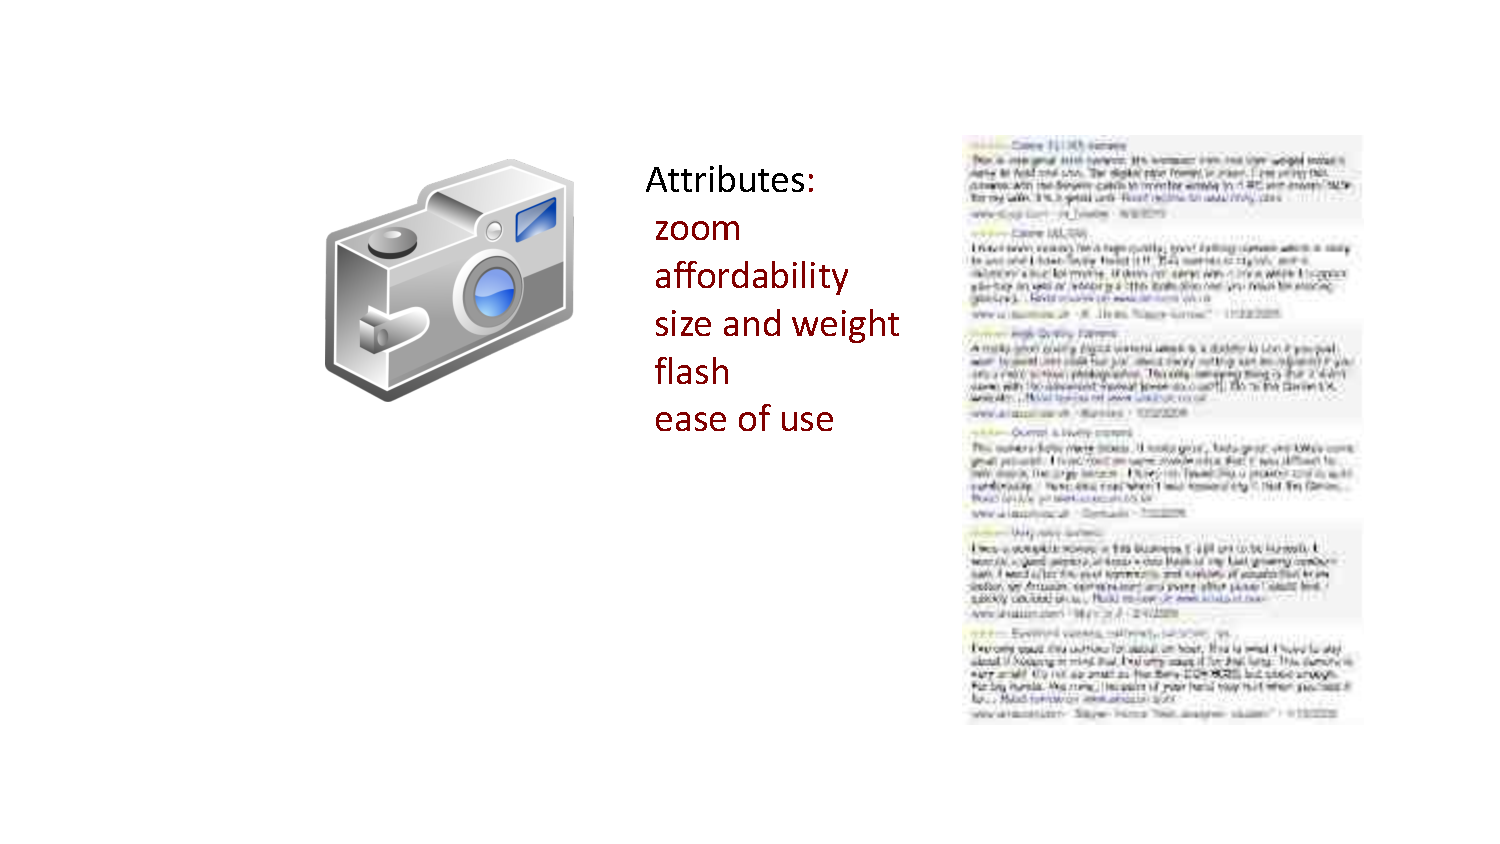
\includegraphics[scale=0.45]{sent1}}
% \only<2>{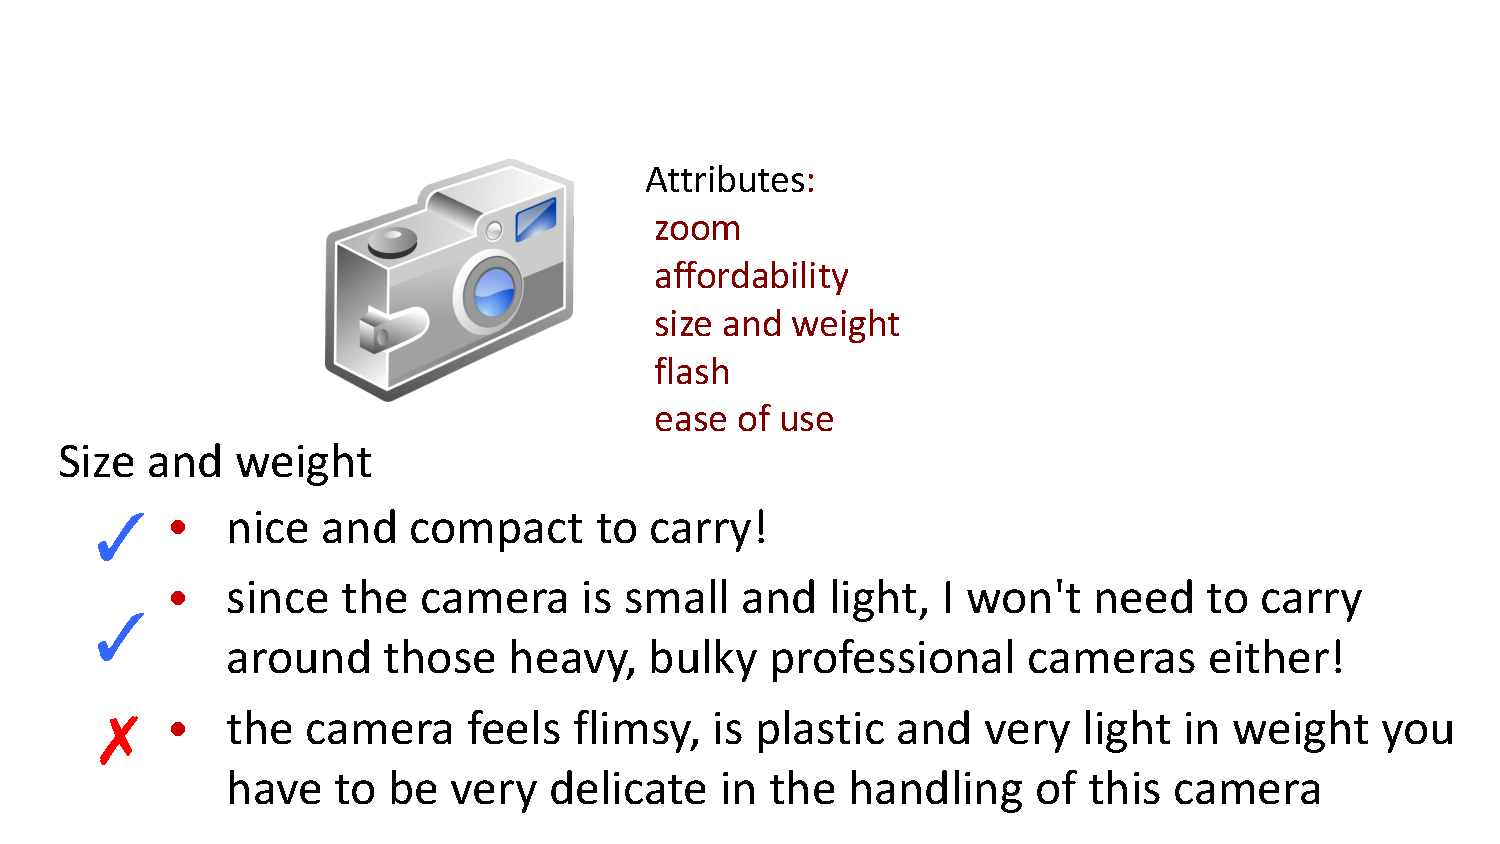
\includegraphics[scale=0.45]{sent2}}
% \only<3>{\hspace{-0.075cm}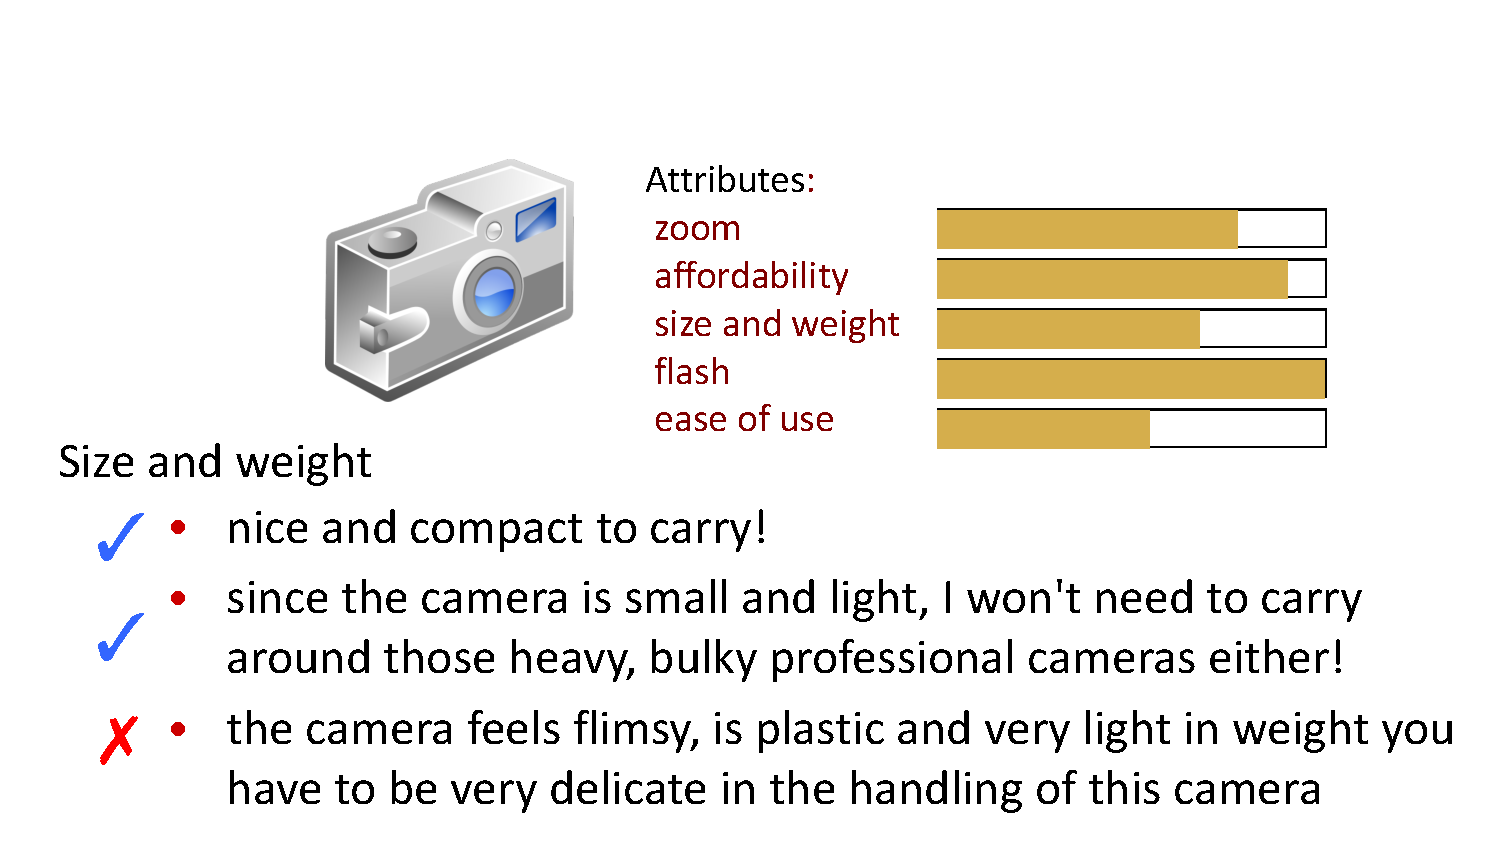
\includegraphics[scale=0.45]{sent3}}
% \end{frame}

% \begin{frame}
% \frametitle{Machine translation}
% \only<1>{\vspace{0.01cm}}
% \only<3-4>{\vspace{-0.21cm}}
% \noindent
% \hspace{-0.8cm}
% \only<1>{\hspace{0.24cm}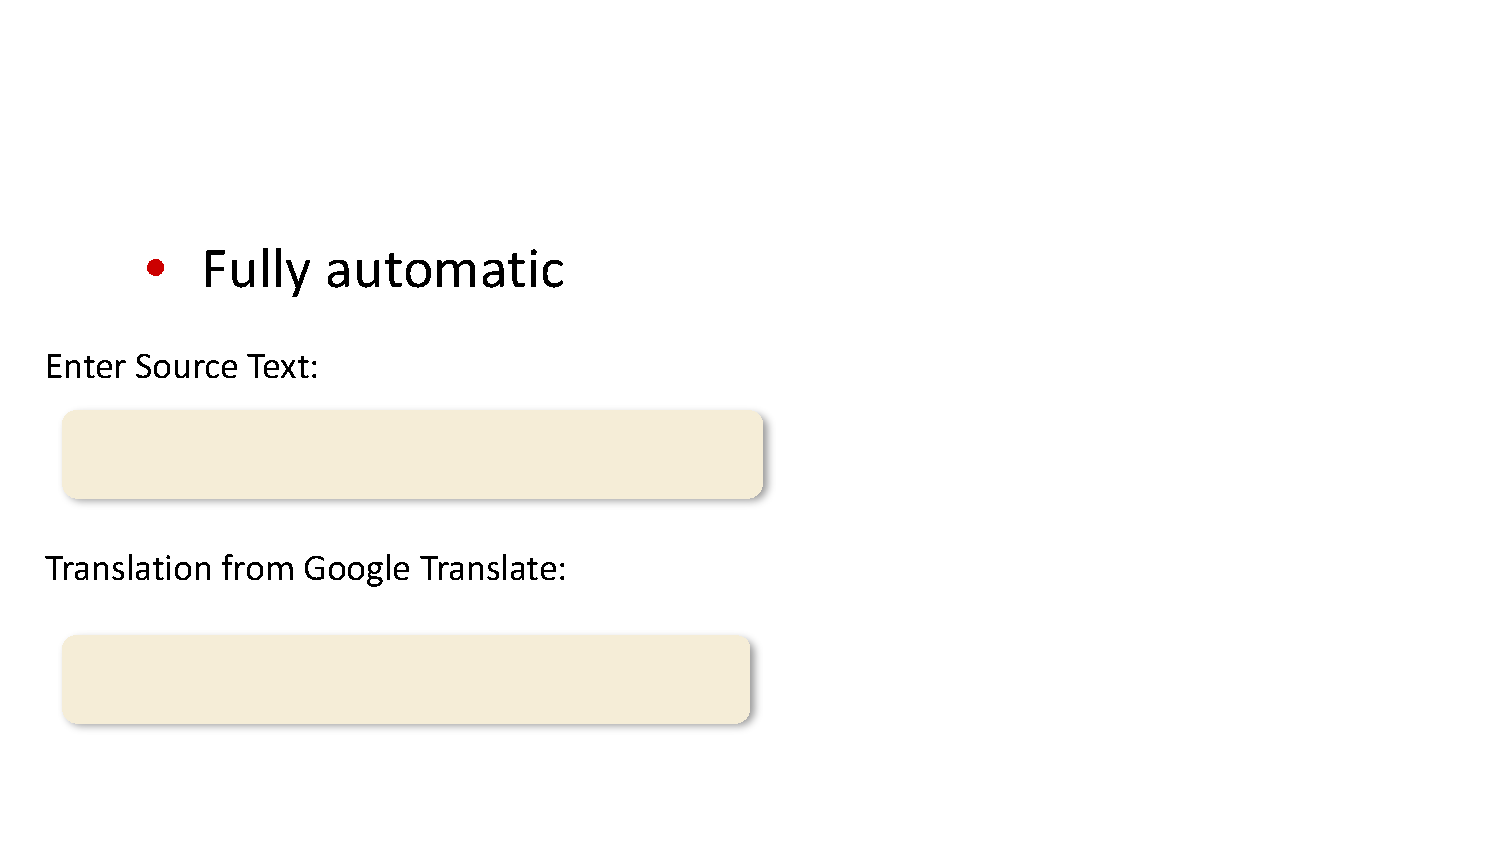
\includegraphics[scale=0.45]{mt1}}
% \only<2>{\hspace{0.16cm}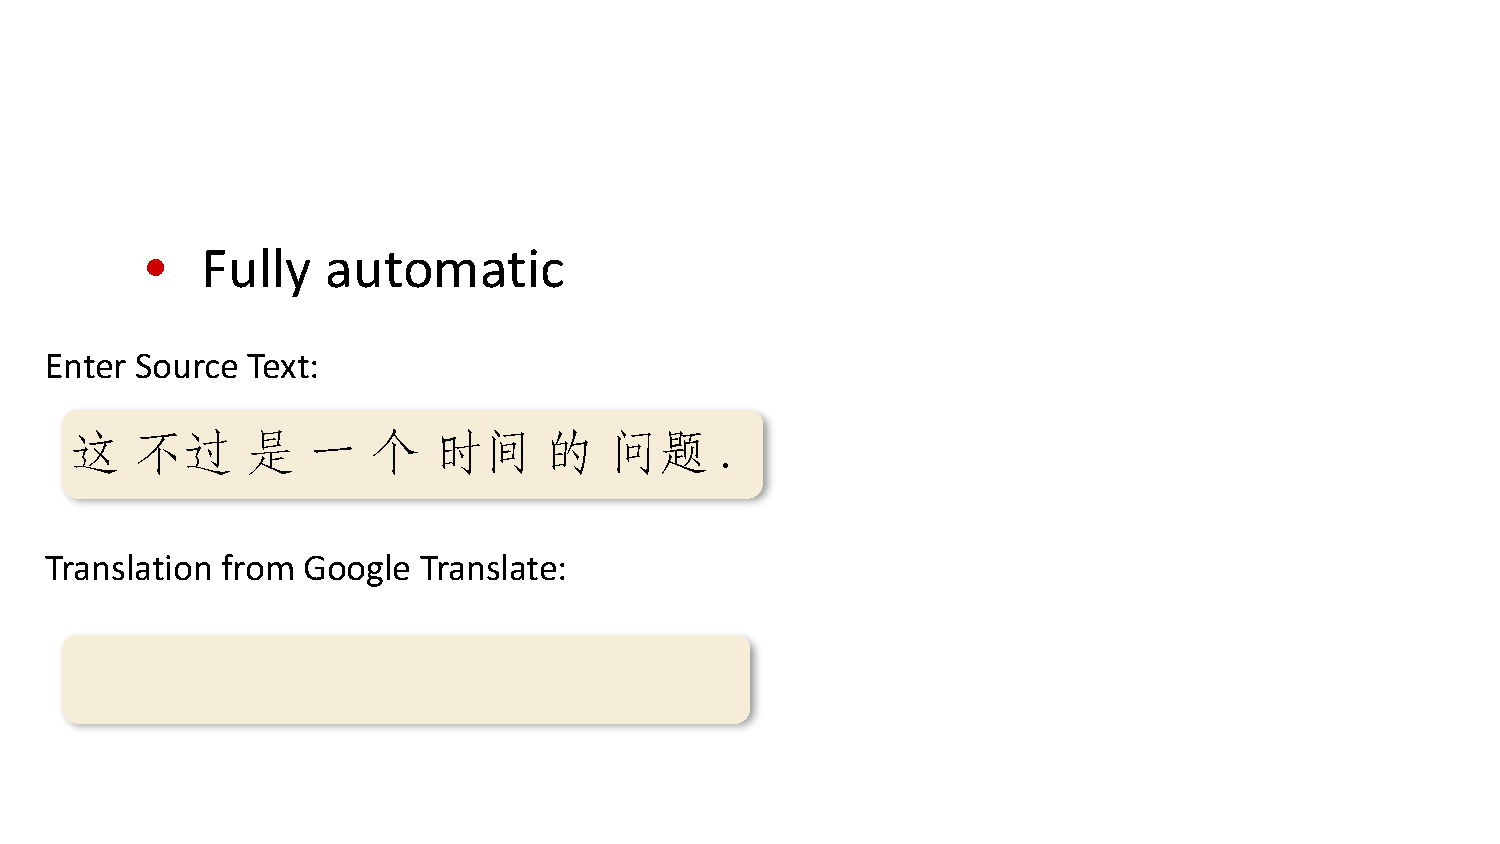
\includegraphics[scale=0.45]{mt2}}
% \only<3>{\hspace{0.07cm}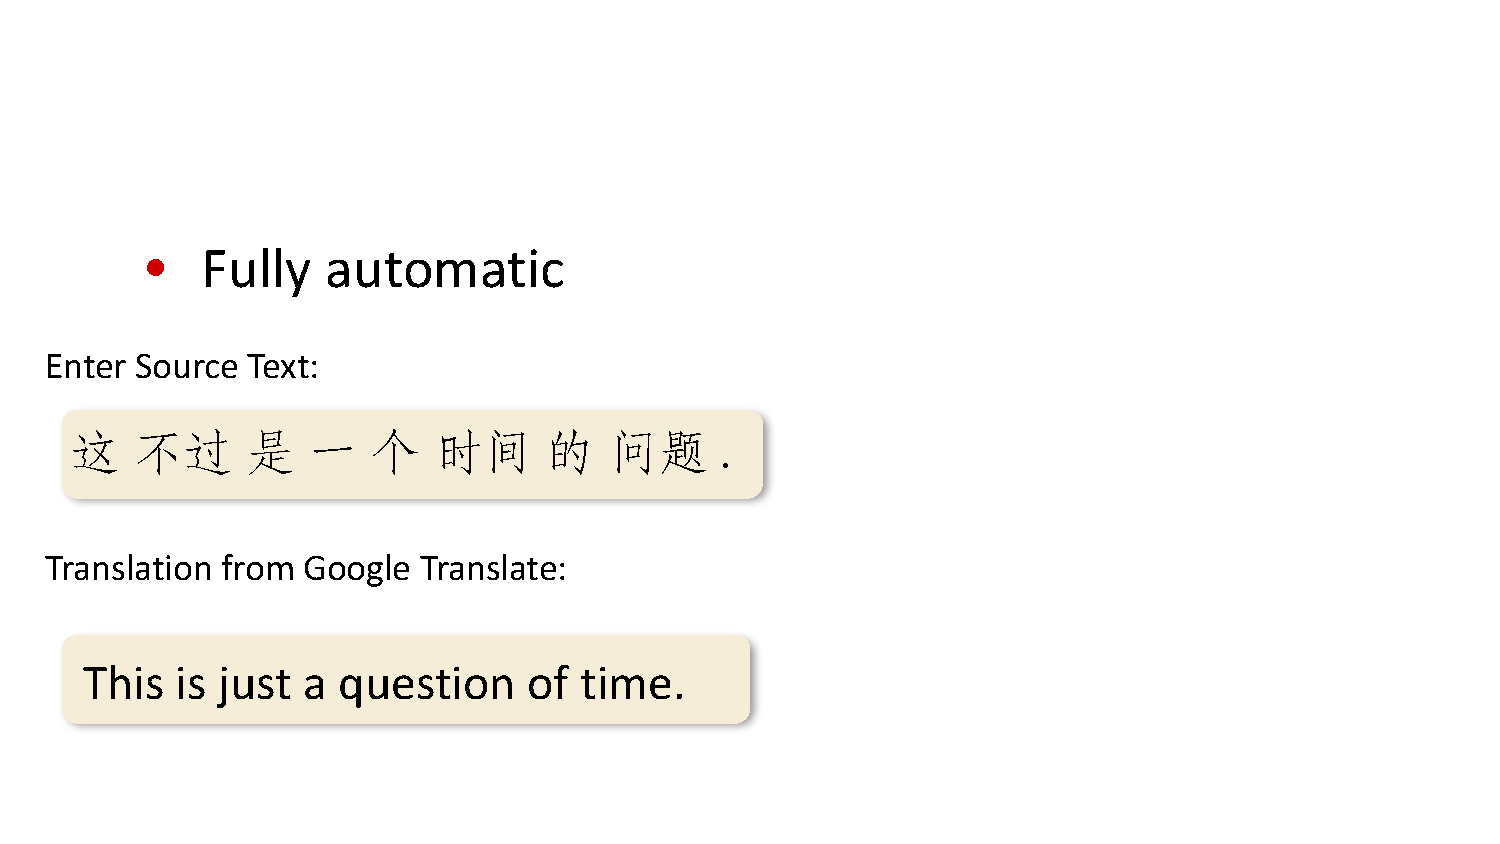
\includegraphics[scale=0.45]{mt3}}
% \only<4>{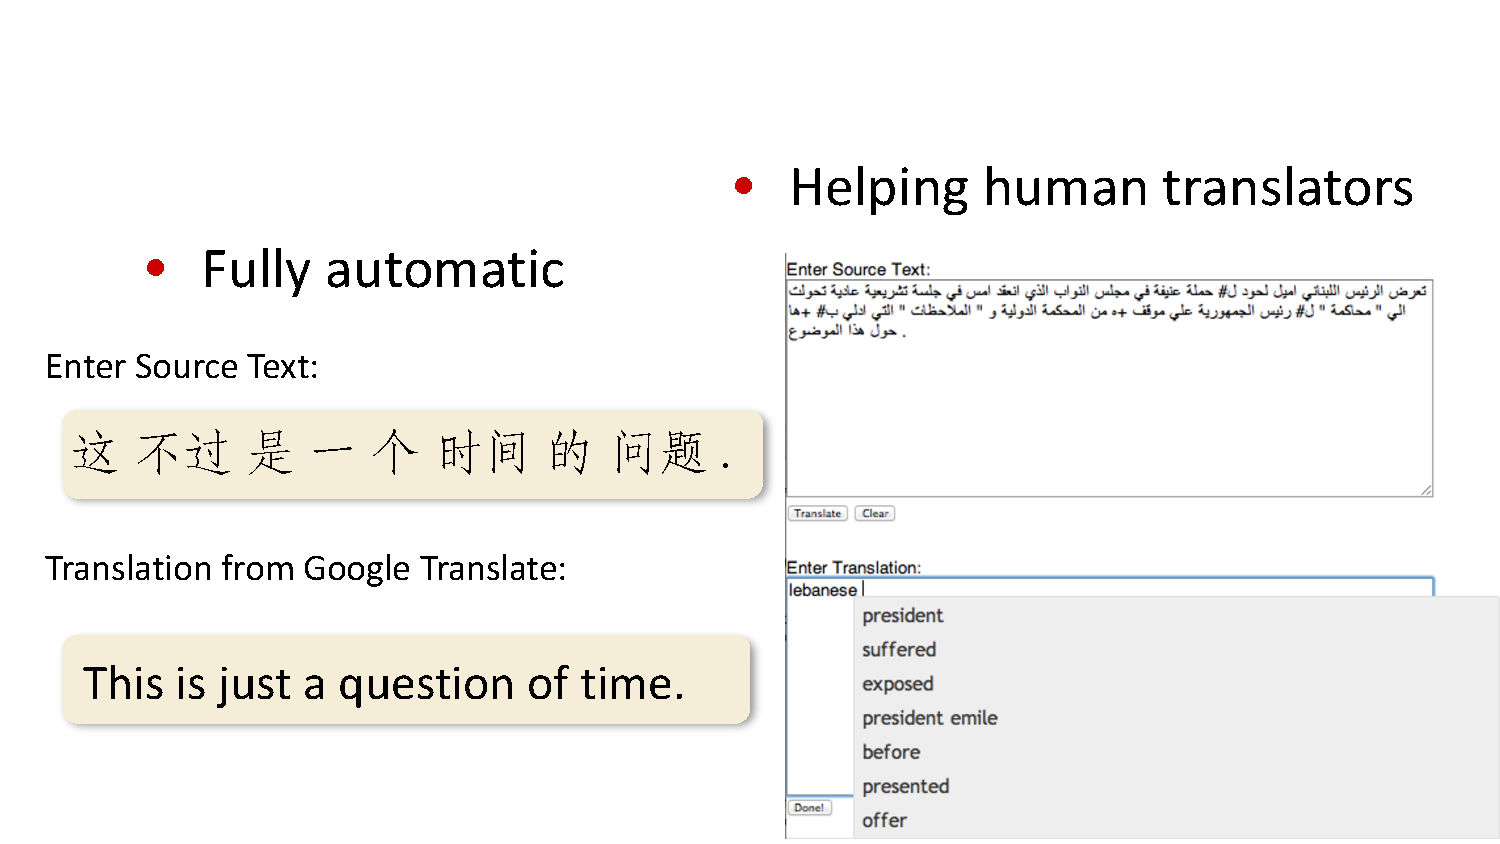
\includegraphics[scale=0.45]{mt4}}
% \end{frame}

\begin{frame}
\frametitle{State of the art}
%\begin{center}
\noindent
\hspace{-1.17cm}
%\begin{tabular}{ccc}
%\includegraphics[scale=0.47]{green} &
%\includegraphics[scale=0.47]{yellow} &
%\includegraphics[scale=0.47]{red} \\
%\end{tabular}
%\end{center}
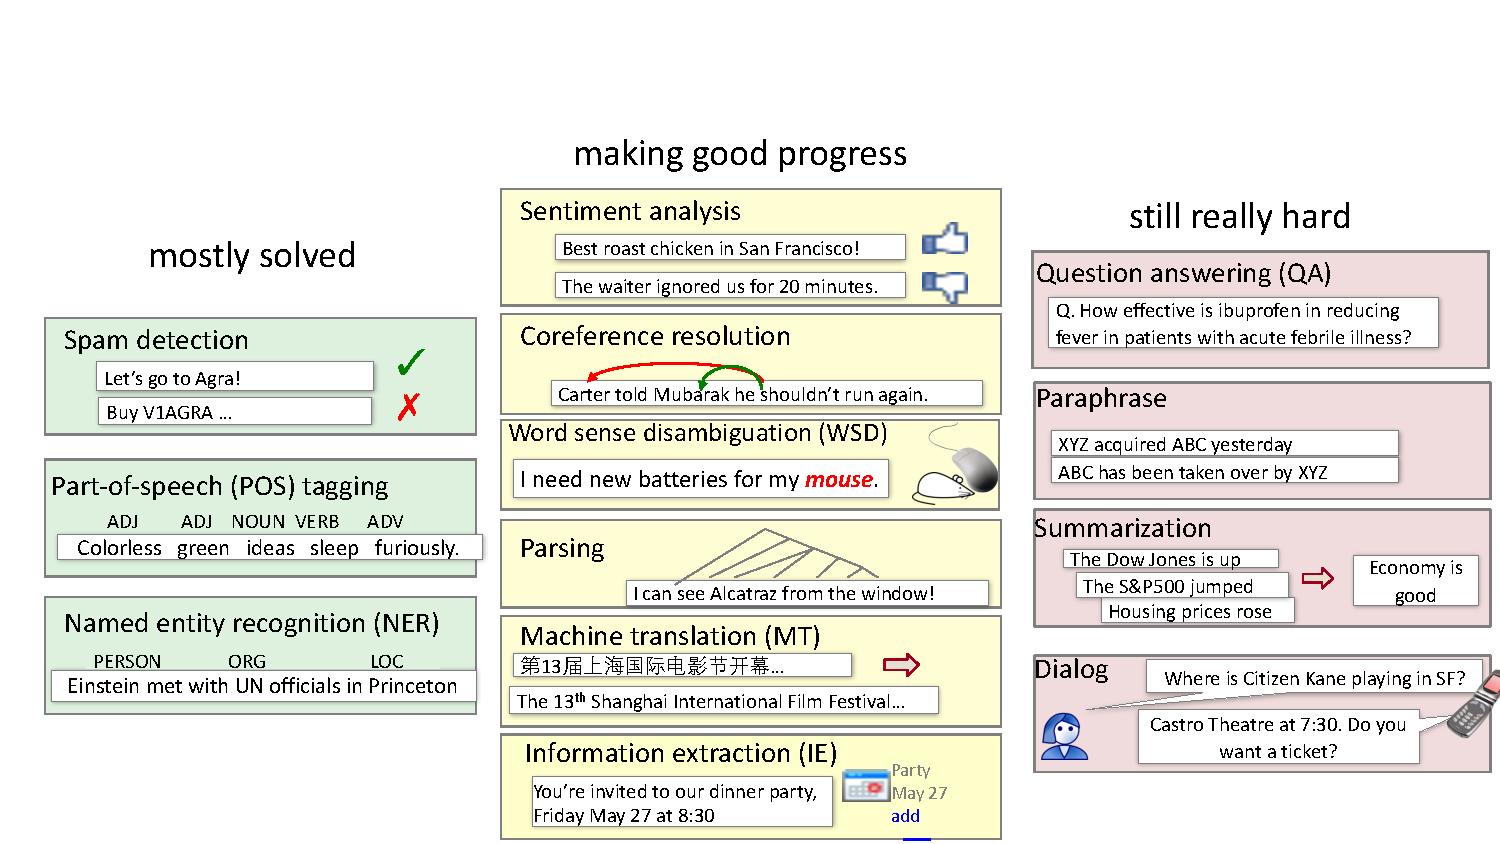
\includegraphics[scale=0.5]{progress}
\end{frame}

\begin{frame}
\frametitle{Ambiguity makes NLP hard}
\hfill

\includegraphics[scale=0.4]{real}

\begin{itemize}
\vspace{-1cm}
\item Teacher strikes idle kids
\item Hospitals are sued by seven foot doctors
\item Red tape holds up new bridges
\item Local high school dropouts cut in half
\item Juvenile court to try shooting defendant  
\end{itemize}
\end{frame}

\begin{frame}
\frametitle{Why else is NLP difficult?}
\noindent
\hspace{-0.65cm}
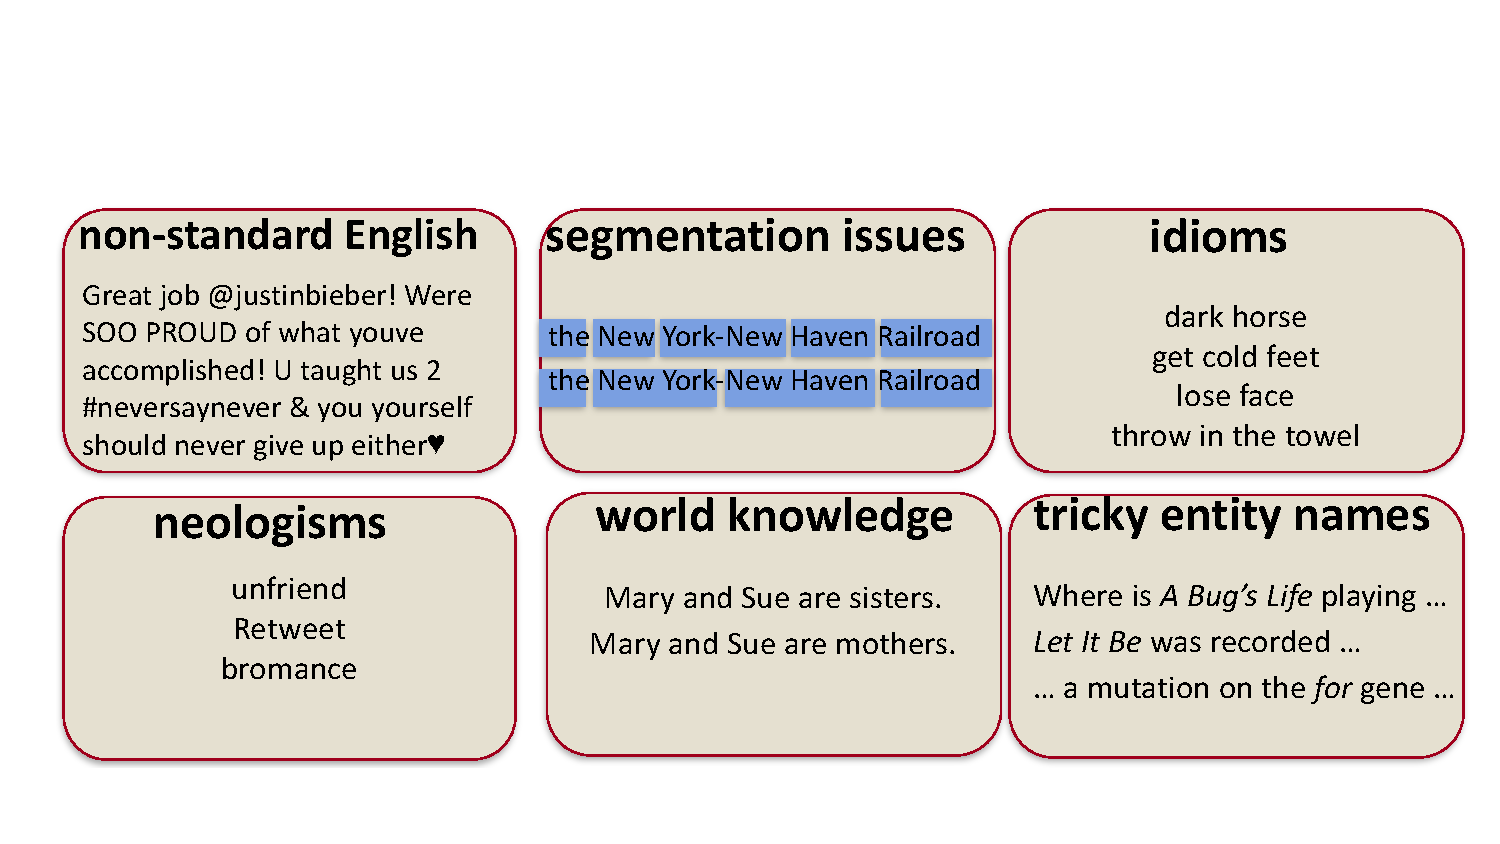
\includegraphics[scale=0.5]{difficulties}
\end{frame}

\begin{frame}
\frametitle{Making progress}
\begin{itemize}
\item What do we need?
\begin{itemize}
\item Knowledge about language
\item Knowledge about the world
\item A way to combine knowledge sources
\end{itemize}
\item State of the art (today):
\begin{itemize}
\item Build statistical models from language data
\item Combine linguistic rules with shallow text features
\item Balance model complexity and computational efficiency
\end{itemize}
\end{itemize}
\end{frame}

\begin{frame}
\frametitle{This course}

\begin{itemize}
\item We focus on key theory and methods for NLP:
\begin{itemize}
\item Regular expressions and finite automata
\item Probability and statistical inference
\item Statistical models of morphology, syntax and semantics
\end{itemize}
\item You should also get an orientation about NLP applications
\item Main textbook: 
\begin{itemize}
\item Jurafsky and Martin, \textcolor{blue}{Speech and Language Processing}
\end{itemize}
\end{itemize}
\end{frame}

\begin{frame}
\frametitle{Flipped-classrom teaching}
\begin{itemize}
\item Traditional (university) teaching:
\begin{itemize}
\item Students are \alert{passive} in the classroom (lectures)
\item Students are \alert{active} on their own (homework, assignments)
\end{itemize}
\item The flipped classroom:
\begin{itemize}
\item Students are \alert{active} in the classroom (problem solving)
\item Students are \alert{passive} on their own (lectures) %but also \alert{active} (quizzes)
\end{itemize}
\item This will be a flipped course:
\begin{itemize}
\item Classroom activity is the key -- and preparation is required
\end{itemize}
\end{itemize}
\end{frame}

\begin{frame}
\frametitle{Scalable Learning}
\begin{itemize}
\item We use a platform called \href{http://www.scalable-learning.com/\#/users/login}{\textcolor{blue}{Scalable Learning}}
\item Students:
\begin{itemize}
\item Create an account and sign up for the course (\alert{enrollment key})
\item Watch lectures and answer quizzes before each class
\item Ask questions personally or anonymously \\(please avoid to hit
  the ``confused'' button)
\item Only explicit questions will be answered
  \\(''\emph{\textcolor{blue}{I don't understand!}}'' is not a
  question)
\end{itemize}
\item Teachers:
\begin{itemize}
\item Check whether students have watched the lectures
\item Check responses to quizzes (anonymously)
\item Answer questions (questions and answers will anonymously be
  displayed to all students)
\end{itemize}
\end{itemize}
\end{frame}

\begin{frame}
\frametitle{Examination and assignments}
\begin{itemize}
\item In-class labs:
  \begin{itemize}
  \item Based on lectures and reading
  \item Work done (mostly) in class
  \item Not to be submitted, will not be assessed
  \end{itemize}
\item<2-> Assignments:
  \begin{itemize}
  \item Based on in-class labs and further reading
  \item Handed in roughly every 1,5 weeks (deadlines on web page)
  \end{itemize}
\item<3-> Survey of an application area:
  \begin{itemize}
  \item Based on a literature survey (2--3 articles)
  \item Oral presentation in class
  \item Written presentation in a term paper (3--5 pages)
  \end{itemize}
\end{itemize}
\end{frame}

\begin{frame}
  \frametitle{Example week schedule I}
  \resizebox{0.85\textwidth}{!}{
    \begin{tabular}{|l|c|c|c|c|c|}
      \hline
      Week 1 &  Monday 6.11& Tuesday 7.11 & Wednesday 8.11& Thursday 9.11& Friday 10.11\\
      \hline
      \multirow{4}{*}{Morning}  &\cellcolor{Maroon!50} & \cellcolor{Green!50}&\cellcolor{Maroon!50}  & \cellcolor{Yellow!50}&\cellcolor{Green!50} \\
      
             &\cellcolor{Maroon!50} & \cellcolor{Green!50}&\cellcolor{Maroon!50}  & \cellcolor{Yellow!50}& \cellcolor{Green!50}\\
             &\cellcolor{Maroon!50} & \cellcolor{Green!50}&\cellcolor{Maroon!50}  &\cellcolor{Yellow!50} & \cellcolor{Green!50}\\  
  & \cellcolor{Maroon!50}\multirow{-4}{*}{Classroom Meeting} & \cellcolor{Green!50}\multirow{-4}{*}{Read Textbook} &\cellcolor{Maroon!50}  \multirow{-4}{*}{Classroom Meeting} & \multirow{-4}{*}{Assignment 1}\cellcolor{Yellow!50}& \multirow{-4}{*}{Read Textbook}\cellcolor{Green!50}\\
  \hline
\multirow{4}{*}{Afternoon} &\cellcolor{Dandelion!60} & \cellcolor{NavyBlue!50} &\cellcolor{Yellow!50} &\cellcolor{Yellow!50} & \cellcolor{NavyBlue!50}\\
&\cellcolor{Dandelion!60} &  \cellcolor{NavyBlue!50}&\cellcolor{Yellow!50} &\cellcolor{Yellow!50} & \cellcolor{NavyBlue!50}\\
&\cellcolor{Dandelion!60} &  \cellcolor{NavyBlue!50}&\cellcolor{Yellow!50} & \cellcolor{Yellow!50}& \cellcolor{NavyBlue!50}\\
& \cellcolor{Dandelion!60}\multirow{-4}{*}{Complete Lab} & \cellcolor{NavyBlue!50} \multirow{-4}{*}{Watch Lectures}& \cellcolor{Yellow!50}\multirow{-4}{*}{Assignment 1} & \cellcolor{Yellow!50}\multirow{-4}{*}{Assignment 1}& \multirow{-4}{*}{Watch Lectures}\cellcolor{NavyBlue!50}\\
  \hline
 \multicolumn{1}{c}{} \\
 \multicolumn{1}{c}{}  \\
\hline
  Week 2 &  Monday 13.11& Tuesday 14.11 & Wednesday 15.11& Thursday 16.11& Friday 17.11\\
  \hline
\multirow{4}{*}{Morning} &\cellcolor{Maroon!50} &\cellcolor{Yellow!50} &\cellcolor{Yellow!50} &\cellcolor{Green!50} & \cellcolor{Maroon!50}\\
&\cellcolor{Maroon!50} & \cellcolor{Yellow!50}& \cellcolor{Yellow!50}&\cellcolor{Green!50} & \cellcolor{Maroon!50}\\
&\cellcolor{Maroon!50} & \cellcolor{Yellow!50}&\cellcolor{Yellow!50} &\cellcolor{Green!50} & \cellcolor{Maroon!50}\\  
  &\cellcolor{Maroon!50} \multirow{-4}{*}{Classroom Meeting} & \cellcolor{Yellow!50}\multirow{-4}{*}{Assignment 1} & \cellcolor{Yellow!50}\multirow{-4}{*}{Assignment 1} & \multirow{-4}{*}{Read Textbook}\cellcolor{Green!50} & \multirow{-4}{*}{Classroom Meeting}\cellcolor{Maroon!50}\\
  \hline
\multirow{4}{*}{Afternoon}&\cellcolor{Yellow!50} &\cellcolor{Yellow!50} &\cellcolor{Yellow!50} & \cellcolor{NavyBlue!50}& \cellcolor{Yellow!50}\\
&\cellcolor{Yellow!50} &\cellcolor{Yellow!50} & \cellcolor{Yellow!50}& \cellcolor{NavyBlue!50}& \cellcolor{Yellow!50}\\
&\cellcolor{Yellow!50} & \cellcolor{Yellow!50}& \cellcolor{Yellow!50}& \cellcolor{NavyBlue!50}& \cellcolor{Yellow!50}\\
&\cellcolor{Yellow!50}\multirow{-4}{*}{Assignment 1} &\cellcolor{Yellow!50} \multirow{-4}{*}{Assignment 1} &\multirow{-4}{*}{Assignment 1}\cellcolor{Yellow!50} &\multirow{-4}{*}{Watch Lectures}\cellcolor{NavyBlue!50}&\cellcolor{Yellow!50} \multirow{-4}{*}{Assignment 1} \\

\hline
\end{tabular}}
\end{frame}

\begin{frame}
  \frametitle{Example week schedule II}
  \resizebox{0.85\textwidth}{!}{
    \begin{tabular}{|l|c|c|c|c|c|}
      \hline
      Week 3&  Monday 20.11 & Tuesday 21.11 & Wednesday 22.11 & Thursday 23.11 & Friday 24.11\\
      \hline
      \multirow{4}{*} {Morning} & \cellcolor{NavyBlue!50} & \cellcolor{Maroon!50}  & \cellcolor{NavyBlue!50}  & \cellcolor{Maroon!50}&\cellcolor{Yellow!50}  \\
            & \cellcolor{NavyBlue!50}& \cellcolor{Maroon!50} &\cellcolor{NavyBlue!50}  & \cellcolor{Maroon!50} & \cellcolor{Yellow!50} \\
            &\cellcolor{NavyBlue!50} & \cellcolor{Maroon!50} &\cellcolor{NavyBlue!50} & \cellcolor{Maroon!50} & \cellcolor{Yellow!50}\\
            & \cellcolor{NavyBlue!50}\multirow{-4}{*}{Watch Lectures} &\cellcolor{Maroon!50}\multirow{-4}{*}{Classroom Meeting} &\cellcolor{NavyBlue!50}\multirow{-4}{*}{Watch Lectures} & \cellcolor{Maroon!50}\multirow{-4}{*}{Classroom Meeting} & \cellcolor{Yellow!50}\multirow{-4}{*}{Assignment 2}\\
      \hline %%%%%%%%%%%%%%%%%%%%%%%%%%%%%%%%%%%%%%%%%%%
      \multirow{4}{*}{Afternoon} &\cellcolor{Yellow!50}  & \cellcolor{Green!50}   & \cellcolor{Yellow!50} & \cellcolor{Green!50} &\cellcolor{Yellow!50}\\
            & \cellcolor{Yellow!50}\multirow{-2}{*}{Assignment 1} & \cellcolor{Green!50}  & \cellcolor{Yellow!50} &\cellcolor{Green!50} &\cellcolor{Yellow!50} \\
      \cline{2-2}
            &\cellcolor{Red} & \cellcolor{Green!50} &\cellcolor{Yellow!50}  & \cellcolor{Green!50} & \cellcolor{Yellow!50}\\
            &\cellcolor{Red}\multirow{-2}{*}{Submit Assignment 1}& \cellcolor{Green!50}\multirow{-4}{*}{Read Textbook}&\cellcolor{Yellow!50}\multirow{-4}{*}{Assignment 2}&\cellcolor{Green!50}\multirow{-4}{*}{Read Textbook}& \cellcolor{Yellow!50} \multirow{-4}{*}{Assignment 2}\\
      \hline
      \multicolumn{1}{c}{} \\
      \multicolumn{1}{c}{}  \\
      \hline
      Week 4 &  Monday 27.11& Tuesday 28.11 & Wednesday 29.11& Thursday 30.11& Friday 1.12\\
      \hline
      \multirow{4}{*}{Morning}& \cellcolor{Green!50} & \cellcolor{Maroon!50} & \cellcolor{NavyBlue!50} & \cellcolor{Maroon!50} &  \cellcolor{Yellow!50}\\
            & \cellcolor{Green!50}&\cellcolor{Maroon!50} & \cellcolor{NavyBlue!50}& \cellcolor{Maroon!50}& \cellcolor{Yellow!50} \\
            & \cellcolor{Green!50}&\cellcolor{Maroon!50} &\cellcolor{NavyBlue!50}  &\cellcolor{Maroon!50} &  \cellcolor{Yellow!50}\\  
            &\cellcolor{Green!50}\multirow{-4}{*}{Read Textbook} &\cellcolor{Maroon!50}\multirow{-4}{*}{Classroom Meeting} &\cellcolor{NavyBlue!50} \multirow{-4}{*}{Watch Lectures}& \cellcolor{Maroon!50}\multirow{-4}{*}{Classroom Meeting}&\multirow{-4}{*}{Assignment 3}  \cellcolor{Yellow!50}\\  
      \hline
      \multirow{4}{*}{Afternoon}& \cellcolor{NavyBlue!50} &  \cellcolor{Yellow!50} &  \cellcolor{Yellow!50}& \cellcolor{Green!50}&  \cellcolor{Yellow!50} \\
            & \cellcolor{NavyBlue!50} &  \cellcolor{Yellow!50}&\multirow{-2}{*}{Assignment 2} \cellcolor{Yellow!50} &  \cellcolor{Green!50}& \multirow{-2}{*}{Assignment 3} \cellcolor{Yellow!50}\\
      \cline{4-4}\cline{6-6}
            & \cellcolor{NavyBlue!50} & \cellcolor{Yellow!50} &\cellcolor{Red} & \cellcolor{Green!50} &\cellcolor{Red} \\
            & \multirow{-4}{*}{Watch Lectures} \cellcolor{NavyBlue!50} &\multirow{-4}{*}{Assignment 2} \cellcolor{Yellow!50}& \cellcolor{Red}\multirow{-2}{*}{Submit Assignment 2} &\multirow{-4}{*}{Read Textbook}  \cellcolor{Green!50}& \multirow{-2}{*}{Submit Survey Proposal}\cellcolor{Red}\\
      \hline
      \multicolumn{1}{c}{} \\
    \end{tabular}
    }
\end{frame}

\begin{frame}
  \frametitle{Example week schedule III}

  \resizebox{0.85\textwidth}{!}{
    \begin{tabular}{|l|c|c|c|c|c|}
      \hline
  Week 5 &  Monday 4.12& Tuesday 5.12 & Wednesday 6.12& Thursday 7.12& Friday 8.12\\
  \hline
\multirow{4}{*}{Morning}& \cellcolor{Green!50} & \cellcolor{Maroon!50} & \cellcolor{NavyBlue!50} & \cellcolor{Maroon!50} &\cellcolor{Yellow!50} \\
       & \cellcolor{Green!50}&\cellcolor{Maroon!50} & \cellcolor{NavyBlue!50}&\cellcolor{Maroon!50} &\cellcolor{Yellow!50} \\
& \cellcolor{Green!50}&\cellcolor{Maroon!50} &\cellcolor{NavyBlue!50} &\cellcolor{Maroon!50} & \cellcolor{Yellow!50}\\  
&\multirow{-4}{*}{Read Textbook}\cellcolor{Green!50} & \cellcolor{Maroon!50}\multirow{-4}{*}{Classroom Meeting}& \cellcolor{NavyBlue!50}\multirow{-4}{*}{Watch Lectures} &\multirow{-4}{*}{Classroom Meeting}\cellcolor{Maroon!50} & \multirow{-4}{*}{Assignment 3}\cellcolor{Yellow!50}\\  
  \hline
\multirow{4}{*}{Afternoon}&\cellcolor{NavyBlue!50} & \cellcolor{Yellow!50}& \cellcolor{Yellow!50}&\cellcolor{Green!50} &\cellcolor{Yellow!50} \\
       &\cellcolor{NavyBlue!50} & \cellcolor{Yellow!50}& \cellcolor{Yellow!50}& \cellcolor{Green!50}&\cellcolor{Yellow!50}\multirow{-2}{*}{Assignment 3} \\
  \cline{6-6}
& \cellcolor{NavyBlue!50} &\cellcolor{Yellow!50}& \cellcolor{Yellow!50} &\cellcolor{green!50} &\cellcolor{Red} \\
       & \multirow{-4}{*}{Watch Lectures}\cellcolor{NavyBlue!50} & \cellcolor{Yellow!50}\multirow{-4}{*}{Assignment 3} &\cellcolor{Yellow!50}\multirow{-4}{*}{Assignment 3} &\cellcolor{Green!50}\multirow{-4}{*}{Read Textbook}& \multirow{-2}{*}{Submit Assignment 3}\cellcolor{Red}\\
  \hline
 \multicolumn{1}{c}{} \\
 \multicolumn{1}{c}{}  \\
  \hline
Week 6 &  Monday 11.12& Tuesday 12.12 & Wednesday 13.12& Thursday 14.12& Friday 15.12\\
  \hline
\multirow{4}{*}{Morning}& \cellcolor{Green!50} &\cellcolor{Maroon!50}  & \cellcolor{NavyBlue!50} & \cellcolor{Maroon!50} &\cellcolor{Yellow!50} \\
       &\cellcolor{Green!50} & \cellcolor{Maroon!50}&\cellcolor{NavyBlue!50} & \cellcolor{Maroon!50}& \cellcolor{Yellow!50}\\
& \cellcolor{Green!50}&\cellcolor{Maroon!50} & \cellcolor{NavyBlue!50} &\cellcolor{Maroon!50} & \cellcolor{Yellow!50}\\  
&\cellcolor{Green!50}\multirow{-4}{*}{Read Textbook} &\cellcolor{Maroon!50}\multirow{-4}{*}{Classroom Meeting} & \cellcolor{NavyBlue!50}\multirow{-4}{*}{Watch Lectures}&\multirow{-4}{*}{Classroom Meeting}\cellcolor{Maroon!50} & \multirow{-4}{*}{Assignment 4}\cellcolor{Yellow!50}\\  
  \hline
\multirow{4}{*}{Afternoon} &\cellcolor{NavyBlue!50} & \cellcolor{Yellow!50}&\cellcolor{Yellow!50} &\cellcolor{Green!50} &\cellcolor{Yellow!50} \\
       & \cellcolor{NavyBlue!50}& \cellcolor{Yellow!50}&\cellcolor{Yellow!50} &\cellcolor{Green!50} & \cellcolor{Yellow!50}\multirow{-2}{*}{Assignment 4}\\
  \cline{6-6}
       &\cellcolor{NavyBlue!50}  &\cellcolor{Yellow!50}& \cellcolor{Yellow!50} &\cellcolor{Green!50} & \cellcolor{Red}\\  
  &\multirow{-4}{*}{Watch Lectures} \cellcolor{NavyBlue!50}& \multirow{-4}{*}{Assignment 4}\cellcolor{Yellow!50} &\multirow{-4}{*}{Assignment 4} \cellcolor{Yellow!50}&\multirow{-4}{*}{Read Textbook}\cellcolor{Green!50}&\multirow{-2}{*}{Submit Assignment 4}\cellcolor{Red} \\
  \hline
\end{tabular}}
\end{frame}

\begin{frame}
  \frametitle{Submission Policy}
  \vspace{-0.6cm}
  \begin{itemize}
  \item We strongly encourage group work in the labs
  \item \textbf{But:} \\assignments must be solved and submitted
    \textbf{\textcolor{red}{individually} (!)}
  \item You will be assessed and graded based on these submissions
  \end{itemize}

  \visible<2->{\textbf{What is Plagiarism?}\vspace{0.2cm}\\
    \emph{\small Plagiarism is the ''wrongful appropriation'' and
      ''stealing and publication'' of another author's ''language,
      thoughts, ideas, or expressions'' and the representation of them
      as one's own original work.}} \visible<3->{(taken from
    http://www.en.wikipedia.org, 2017-03-24)}\vspace{0.2cm}\\
  \visible<4->{\href{https://www.roanoke.edu/Documents/AcademicAffairs/Types\_of\_Plagiarism.pdf}{$\rightarrow$ \textcolor{blue}{Examples}}}\vspace{0.2cm}\\
  \visible<5->{\href{http://www.uu.se/en/students/your\_rights/cheating/}{\textbf{$\rightarrow$ UU's policy and overview of your rights}}
  }
\end{frame}



\begin{frame}
\frametitle{Examples for Real-World Applications}
\hfill 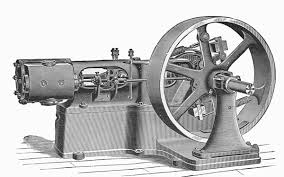
\includegraphics[scale=0.4]{steam}
\begin{itemize}
\vspace{-2.5cm}
\item Machine translation
\item Information retrieval
\item Information extraction
\item Sentiment analysis
\item Summarization
\item Question answering
\item Dialogue systems
\item Language tutoring systems
\item Proofreading tools
\end{itemize}
\end{frame}

\begin{frame}
\frametitle{Programming}
\begin{itemize}
\item Basic programming skills is a prerequisite for the course
\item For in-class labs we will mainly use \textcolor{blue}{Python}
\begin{itemize}
\item You don't need to know Python to take the course
\item But you need to know how to run a Python program
\item And you will probably learn some Python in the process
\end{itemize}
\item In principle, you can use any programming language you like
\end{itemize}

\end{frame}

\begin{frame}
\begin{center}
{\huge {\bf Questions?}}
\end{center}
\end{frame}

\end{document}


